% vim: set spell spelllang=en tw=100 et sw=4 sts=4 :

\documentclass[20pt,a1paper,landscape]{tikzposter}

\usepackage{complexity}
\usepackage{wrapfig}
\usepackage{microtype}

\usepackage{lmodern}
\renewcommand*\familydefault{\sfdefault}
\usepackage[T1]{fontenc}

\title{Solving Hard Problems by Counting and Colouring Things In}
\author{Ciaran McCreesh and Patrick Prosser}
\institute{University of Glasgow, Glasgow, Scotland}
\titlegraphic{
\includegraphics[keepaspectratio=true,scale=2]{UoG_keyline.eps}}

\settitle{
    \begin{tikzpicture}
        \node (T) [inner sep=0pt] {\begin{minipage}{\linewidth}
                \color{titlefgcolor}
                {\bfseries \Huge \hspace{10mm}\@title \par}
                \vspace*{1em}
                {\Large {\bfseries \hspace{10mm}\@author}, \@institute}
        \end{minipage}};

        \node at (T.east) [anchor=center, inner sep=0pt, xshift=-8cm] {\@titlegraphic};
    \end{tikzpicture}
}

% University of Glasgow standard colours

\definecolor{uofgblue}{rgb}{0, 0.321569, 0.533333}
\colorlet{uofgblue20}{uofgblue!20!white}
\colorlet{uofgblue40}{uofgblue!40!white}
\colorlet{uofgblue60}{uofgblue!60!white}
\colorlet{uofgblue80}{uofgblue!80!white}

\definecolor{uofgstone}{rgb}{0.498039, 0.454902, 0.403922}
\colorlet{uofgstone40}{uofgstone!40!white}

\definecolor{uofgtdarkgreen}{rgb}{0.380392, 0.564706, 0.501961}
\definecolor{uofgtlightgreen}{rgb}{0.615686, 0.788235, 0.729412}
\definecolor{uofgtyellow}{rgb}{0.85098, 0.827451, 0.643137}
\definecolor{uofgtorange}{rgb}{0.784314, 0.694118, 0.545098}

\definecolorstyle{UofG}{
}{
    % Background Colors
    \colorlet{backgroundcolor}{uofgstone}
    \colorlet{framecolor}{black}
    % Title Colors
    \colorlet{titlefgcolor}{white}
    \colorlet{titlebgcolor}{uofgblue}
    % Block Colors
    \colorlet{blocktitlebgcolor}{white}
    \colorlet{blocktitlefgcolor}{uofgblue}
    \colorlet{blockbodybgcolor}{white}
    \colorlet{blockbodyfgcolor}{black}
    % Innerblock Colors
    \colorlet{innerblocktitlebgcolor}{uofgblue}
    \colorlet{innerblocktitlefgcolor}{black}
    \colorlet{innerblockbodybgcolor}{uofgstone}
    \colorlet{innerblockbodyfgcolor}{black}
    % Note colors
    \colorlet{notefgcolor}{black}
    \colorlet{notebgcolor}{uofgtyellow}
    \colorlet{noteframecolor}{red}
}

\usetheme{Autumn}
\usecolorstyle{UofG}

\tikzposterlatexaffectionproofoff

\useblockstyle[bodyverticalshift=-1cm, roundedcorners=1]{Default}

\renewcommand{\Huge}{\fontsize{61.92}{77}\selectfont}

% Styles for drawings

\tikzset{edge/.style={line width=3pt, color=uofgstone}}

% Colours for the graph lines

\colorlet{gp lt color 0}{uofgblue}
\colorlet{gp lt color 1}{uofgblue60}
\colorlet{gp lt color 2}{uofgblue20}
\colorlet{gp lt color 3}{uofgtorange}

\begin{document}
\maketitle

{
    \colorlet{blockbodybgcolor}{uofgtyellow}
    \colorlet{blocktitlebgcolor}{uofgtyellow}
    \block[bodyverticalshift=0cm, bodyinnersep=3mm]{}{
        \centering\begin{minipage}{0.94\textwidth}
            \textbf{Combinatorics} is a branch of mathematics devoted to counting and colouring
            things in while respecting certain rules, and \textbf{Combinatorial Optimisation} is
            about finding the ``best'' way to do this. Some important real-world problems can be
            reduced to combinatorial optimisation problems, which makes them easier to model and
            solve using computers. Our research investigates exploiting \textbf{multi-core
            parallelism} to speed up the solving process.
        \end{minipage}
    }
}

\begin{columns}
\column{0.38}

\block{Minimising Resource Usage, with Constraints}{
\begin{wrapfigure}[10]{r}{0.38\linewidth}
    \begin{center}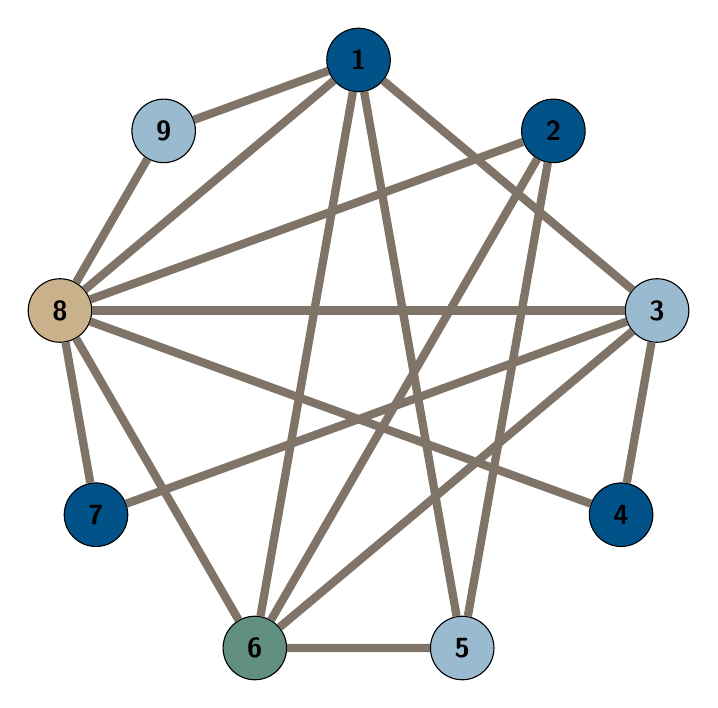
\begin{tikzpicture}[scale=1.75]%{{{
        \newcount \c
        \foreach \n in {1, ..., 9}{
            \c=\n
            \multiply\c by -40
            \advance\c by 130

            \ifthenelse{\n = 1 \OR \n = 2 \OR \n = 4 \OR \n = 7}{
                \node [draw, circle, fill=uofgblue, inner sep=5pt, font=\bfseries] (N\n) at (\the\c:2.2) {\n};
            }{
                \ifthenelse{\n = 3 \OR \n = 5 \OR \n = 4 \OR \n = 7 \OR \n = 9}{
                    \node [draw, circle, fill=uofgblue40, inner sep=5pt, font=\bfseries] (N\n) at (\the\c:2.2) {\n};
                }{
                    \ifthenelse{\n = 6}{
                        \node [draw, circle, fill=uofgtdarkgreen, inner sep=5pt, font=\bfseries] (N\n) at (\the\c:2.2) {\n};
                    }{
                        \node [draw, circle, fill=uofgtorange, inner sep=5pt, font=\bfseries] (N\n) at (\the\c:2.2) {\n};
                    }
                }
            }
        }

        \draw [edge] (N1) -- (N5); \draw [edge] (N1) -- (N9);
        \draw [edge] (N2) -- (N5); \draw [edge] (N2) -- (N6); \draw [edge] (N2) -- (N8);
        \draw [edge] (N3) -- (N4); \draw [edge] (N3) -- (N7);
        \draw [edge] (N4) -- (N8);
        \draw [edge] (N5) -- (N6);
        \draw [edge] (N7) -- (N8);
        \draw [edge] (N8) -- (N9);

        \draw [edge] (N1) -- (N3);
        \draw [edge] (N6) -- (N8);
        \draw [edge] (N1) -- (N6);
        \draw [edge] (N1) -- (N8);
        \draw [edge] (N3) -- (N6);
        \draw [edge] (N3) -- (N8);
    \end{tikzpicture}\end{center}
\end{wrapfigure}

Suppose we need to \textbf{schedule a day's meetings}. If a person needs to attend both meeting 3
and meeting 6, then these two meetings cannot be held at the same time. We can model this as a graph
problem: we draw a circle for each meeting, and put a line between two circles if these two meetings
must occur at different times. We then want to colour in these circles, giving adjacent circles
different colours, and using as few colours as possible. By treating different colours as different
time slots, colouring in the graph gives us an optimal meeting schedule.

\medskip

We can handle richer constraints: we might have a limit on how many circles any colour can be used
in (if we only have a \textbf{limited number of meeting rooms}), or we might want each colour to be
used on the same number of circles (for a \textbf{balanced workload}).

\medskip

More generally, graph colouring tells us how to use \textbf{as few resources as possible},
respecting conflicts. Industrial uses include call centre staff allocation, scheduling jobs on
machinery, radio bandwidth allocation, and reducing the impact of vehicle maintenance.
}

\block{Finding Interesting Patterns}{
    More generally, the \textbf{maximum common subgraph} problem allows us to see how similar two
    graphs are, by identifying a large pattern common to both graphs. This is useful in biochemistry
    and in drug design.
}

\column{0.38}

\block{Finding Large, Interconnected Groups of People}{
    Finding cliques lets us select \textbf{as much of a resource as possible}, respecting
    compatibility rules. Clique-finding algorithms have been used to improve the reliability of
    communications and networking protocols, for social media analysis, for verifying electronic
    circuits, and for controlling flying robots.
}

\block{More Flexibility via Constraint Programming}{

Large-scale industrial successes for constraint programming include scheduling airport gate and crew
allocations, optimising vehicle deliveries, reducing production costs in lumber processing,
producing greener and more energy-efficient data centres, scheduling the Rosetta / Philae mission
operations, reducing the cost of an invasion, and organising sporting seasons for optimal TV
coverage.
}

\column{0.24}
\block{Research Goals}{
    Combinatorial optimization is, in general, a \textbf{hard problem} (like the famous
    \textbf{travelling salesman problem}): every additional variable we add in can double the
    difficulty of finding a solution, so the time taken to solve a problem grows exponentially. In
    practice we can usually avoid this worst case, but solving these problems still takes longer
    than we would like.

    \medskip

    Modern processors have at least two, and sometimes as many as fifteen, processing cores. We
    might hope that we could use these cores to make our programs \textbf{run faster},
    or at least to allow us to \textbf{solve larger problems} in the time we have.

    \medskip

    In general, we do this by splitting problems up into evenly sized, independent pieces of work,
    which may be evaluated independently in parallel. Unfortunately combinatorial optimisation
    problems tend to be \textbf{highly irregular} (cannot be split into evenly sized pieces) and
    require \textbf{speculative parallelism} (the pieces have dependencies upon each other, and we
    must guess what the answer might be allow parallel evaluation).

    \medskip

    Despite this, results can be favourable. Our approach uses parallelism to explicitly
    \textbf{introduce diversity} into a search process to offset the weakest choices made by
    heuristics, so our parallel workers are reducing our commitment to potentially costly early
    mistakes. This is combined with late rebalancing, to give good work balance with low overheads
    and good scalability.
}

\block[bodyverticalshift=0cm]{}{
    \texttt{c.mccreesh.1@research.gla.ac.uk}

    \smallskip
    \small
    This work was supported by the Engineering and Physical Sciences Research Council [grant number
    EP/K503058/1]
}

\end{columns}

\end{document}

